\documentclass[11pt]{report}
\listfiles

\usepackage[colorlinks]{hyperref}
 \usepackage{glossaries} % acronym will go in main glossary
 %\usepackage[acronym]{glossaries} % make a separate list of acronyms

\makeglossaries
\usepackage{graphicx}
\setcounter{secnumdepth}{5}
\setcounter{tocdepth}{5}
\begin{document}

\begin{titlepage}

\begin{center}


% Upper part of the page

\includegraphics[scale=1.0]{images/logo.png}

\textsc{\LARGE University of Western Ontario}\\[1.5cm]

\textsc{\Large Software Specifications: Camera Simulation Environment}\\[0.5cm]


% Title
{ \huge \bfseries Version 0.01}\\[0.4cm]

% Author and supervisor
\begin{minipage}{0.4\textwidth}
\begin{flushleft} \large
\emph{Author:}\\
Kartik \textsc{Thakore} \\
kthakore@uwo.ca 
\end{flushleft}
\end{minipage}
\begin{minipage}{0.4\textwidth}
\begin{flushright} \large
\emph{Supervisors:} \\
Dr.~Hanif \textsc{Ladak}\\
Dr.~Terry \textsc{Peters} 
\end{flushright}
\end{minipage}

\vfill

% Bottom of the page
{\large \today}

\end{center}

\end{titlepage}
\bibliographystyle{IEEE}
\nocite{*}

\tableofcontents

\newpage 

\chapter{Introduction}
  
A core component of Medical Imaging application is the use of computer vision. Camera calibration is a common task required for computer vision. Camera calibration can be a difficult task for researchers without prior graphics background. Cameras have been model in extensive literature that model, and thus can be simulated. A virtual environment would provide a activity based learning approach for camera calibration. 
     
\section{Overview}

\newacronym[\glsshortpluralkey=VR]{VR}{VR}{Virtual Reality: is a simulated environment that is implemented to provide a simulated experience of a real world process or activity}

     
\begin{enumerate}
\item A virtual reality (\glsname{VR}) environment that simulates extrinsic and intrinsic parameters of a camera will provide a sufficient model to allow training on transformation matrices involved with camera calibration.
\item Camera calibration of a simple camera system, performed with prior training in a virtual reality environment, will yield insignificantly different capture camera parameters with real world camera system. 
\end{enumerate}

As a first step software specifications will be developed based on interviews with graduate supervisors. The preliminary specifications will need to be updated in an iterative fashion. 

\section{Background and Significance}

Medical Imaging tasks such as image fusion, registration, feature tracking, etc. are built on the understanding of the mathematical concepts of vision systems. Computer vision is an increasing component of image-guided interventions. Moreover it is often difficult for researchers not from a computer vision background to learn quickly. Virtual environments that simulate computer vision systems would both hasten the learning curve and also act as a prototyping environment for new applications of video-based technology in image-guided interventions. 

\newglossaryentry{pcm}{name={Pinhole Camera Model},
description={The pinhole camera model defines a camera as a mathematical relation between the coordinates of a 3D point, projected onto an image plane. This is also called the Perspective Model. It is a common camera model used in computer vision}}


Mathematically, vision systems can be represented as matrices that perform operations on a spatial field. Cameras in medical imaging essentially transform three-dimensional content to two-dimensional planes (\gls{pcm} \cite{CV}). Thus, locations in 2D images correspond to the position and orientation of objects in the real world.

To be able to capture the position and orientation of objects, a transformation matrix is required from the 2D images. This transformation matrix is acquired by performing camera calibration. Calibration involves acquiring images of known objects with known positions and orientations in the real space. Next, feature points are selected on the 2D image. The selection of feature points are done either manually or using libraries such as OpenCV. The correspondence sets up the transformation between the real world coordinate system and the image coordinates.

Simulation of this process can begin by modeling the camera using the perspective projection model. The model can be represented in matrix notation as:

\begin{equation} s * p = A * [R|t] * P  \end{equation}
 
where  \[A\] is defined as the intrinsic matrix, \[s\] represents the arbitrary scale factor, \[p\] are the 2D image coordinates, \[P\] are the corresponding 3D world coordinates, and finally \[[R|t]\] are the extrinsic parameters.

The intrinsic matrix can be calculated from camera dependent parameters such as focal length and CCD pixel. Additionally, the extrinsic parameters are user defined such that rotation and translation are selected by the user. Finally, the \[P\] world coordinates are simply defined by the user and the scene that will rendered in the virtual reality environment. 

A key challenge faced by graduate students in areas such as image-assisted surgery is in learning the calibration process and understanding the sensitivity of the calibration results on estimated parameters. Indeed, experience at the Robarts Research Institute indicates that students can take several months to learn about camera calibration. Simulation will allow for applications such as training and prototyping. 

\newglossaryentry{SIT}{name={SIT},
description={System Integration Testing, test the overall system via, given inputs and expect outputs}}

\newglossaryentry{UAT}{name={UAT},
description={User Acceptance Testing, tests the system to ensure the user experience and expectations are met}}

Once the software system is developed, System Integration Testing (\glsname{SIT}) will be performed. Additionally, validation will be performed with User Acceptance Testing (\glsname{UAT}) of a selected group of volunteers. 

The implementation will depend essentially on prior work done in Dr. Peters lab with image-guided surgery. Additional resources will be leverage in Image processing and computer vision from Dr. Ladak's work. Specifically projects that depend heavily on calibration of camera systems for medical applications have analyzed to develop specifications for the simulator \cite{CC}. 
 

\section{Relevance}

Camera calibration is a difficult task and a widely recurrent task at Robart's Research Institute in Medical Imaging. Additional camera calibration is a means to an end in most projects and not the focus. The essential tasks involved for performing a camera calibration are similar across projects with potential for standardization and collaboration. In Dr. Peters' laboratory, a considerable amount of effort is placed in camera calibration in several research projects. Each project involves isolated or loosely collaborated work on camera calibration. No software currently exists to help with training of camera collaboration. 

Selecting a camera is crucial to a medical imaging application. A virtual environment may help to explore and compare various camera systems based on parameters provided by manufacturers. Allowing researchers to objectively try systems rather then purchasing each system and performing manual calibration. This will facilitate prototyping and will be a boon for researchers in  gaining an intuitive understanding into the critical factors of camera calibration and the impact on their application. 

\section{Scope}
The scope of this project is primarily to create a virtual environment that can reasonably simulate common cameras used in medical applications. The system will be able to create cameras given parameters that can be used to view a scene and run camera calibration tests on. Once calibrated, the system will allow the user to capture virtual images. 
 
\begin{enumerate}
\item Develop a \glsname{VR} environment that can calculate transformation matrices based on given locations, poses, and camera parameters.  
\item Implement a \glsname{VR} environment that simulates camera calibration within user specified scenes. Develop an online tool that can be accessed by a wide audience in the medical imaging field.
\end{enumerate}

\section{Technical Overview}

\subsection{User Interface}

\newglossaryentry{webb}{name={Web Browser},
description={A cross platform software package to view HTTP provided content from service providers}}

\newglossaryentry{Javascript}{name={Javascript},
description={A cross platform scripting language that runs on \glsname{webb}}}

\newglossaryentry{HTML5}{name={HTML5}, description={Is the fifth version of the Hypertext Markup Language that provides many new features such as canvas and web sockets}}
\newglossaryentry{WebGL}{name={WebGL}, description={A web technology being developed by the Khronos Group to bring accelerated graphics to the web browser, on a canvas}}

One of the initial aim of this project was to provide a easily distributed user interface. A web interface is a proven technology in providing distributed interfaces. The user interface provided by this system will be designed on a \glsname{HTML5}/\glsname{WebGL} project that will work over pre-specified \glsname{webb}. \glsname{WebGL} sits on top of \glsname{HTML5}'s canvas feature and will provide 3D rendering capabilities on enabled \glsname{webb}. Most user demographics are familiar with using a \glsname{webb}, which makes this a viable option. 

\glsname{WebGL} will be written in the \glsname{Javascript} language that is a platform provided by most mordern \glsname{webb}. 

An alternative option involves creating custom distribution and front end software ( similar to a \glsname{webb} ). This is not feasible with the time frame for a Masters project. 

\subsection{Application Server}

\newglossaryentry{app}{name={Application Server},
description={An web service provider that responds to requests from the \glsname{webb}}}

An \glsname{app} will be built to provide the \glsname{Javascript} and \glsname{HTML5} documents to the \glsname{webb}. Additionally, the server will utilize middleware platforms that help to scale (ensure the \glsname{app} responds to varying amounts of requests from multiple \glsname{webb}s).

\subsubsection{HTTP Server}

\newglossaryentry{HTTP}{name={HTTP}, description={ HyperText Transport Protocol defines the protocol of transporting documents to a web client}}

The \glsname{HTTP} Server will be reponsible for responding to requests sent by \glsname{webb} clients. The key requirement required of the \glsname{HTTP} Server is to scale reasonably with an increase in demands. Most of the computational expense will be done on the \glsname{webb} client, due to the way \glsname{WebGL} works. Therefore a scalable \glsname{HTTP} Server will ensure that the response for the \glsname{WebGL} and \glsname{HTML5} documents are provided in a timely manner. For this reason the Nginx \glsname{HTTP} Server and a Starman/PSGI middleware server will be used.

\subsubsection{Dispatch/Controller}

\newglossaryentry{OpenCV}{name={OpenCV}, description={A software library that has a camera calibration component.}}

The user will be using the system to do camera calibration that will require a interface between the frontend and \glsname{OpenCV} features. A controller will be used to define to protocol by which the frontend will communicated with the \glsname{OpenCV} Server. 

\subsubsection{OpenCV Server}

This server will provide the \glsname{app} with \glsname{OpenCV} features such as camera calibration and re-projection of calibration grids.

\chapter{User Specifications}

This chapter defines the user of this system and their specifications. Defining the user ensure that the system can be designed with a \glsname{UAT} goal in mind. 

\begin{figure}[htp]
\centering
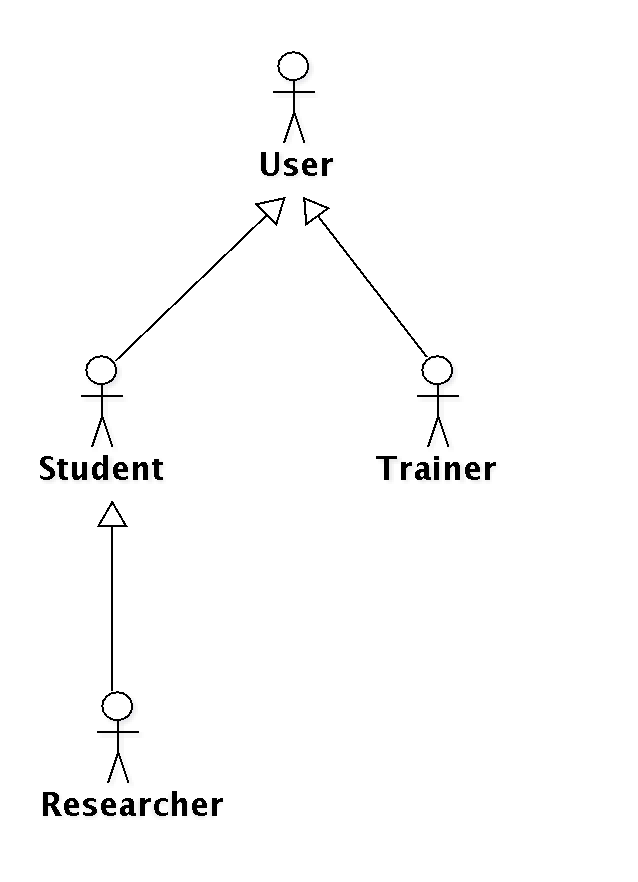
\includegraphics[scale=0.25]{images/UserOverview.png}
\caption{Users}
\label{fig:uo}
\end{figure}

\section{Users} 

The system user is a generalization of several other users as depicted in the use case diagram \ref{fig:uo}.  

\subsection{Student}

The student user is the primary user of the system. This system is essentially made to facilitate the understanding of the student user. Student users are defined as any user that needs to learn and work with camera transformation.  

\subsubsection{Researcher}

The student user can also be extended as a researcher who needs a deeper understanding of camera calibration for a research project. These project involve camera calibration as a critical component in the implementation. 

\subsection{Trainer}

Another user that may use the system is the trainer. Trainer users use the system as a guide for students and researcher. The direct requirements of the trainer user needs to be captured at a later date.

\section{Use Cases}

Use Cases define the process the system will take to meet the needs of the users. Each use case is written in a list format showing what the user will see and react with during the specific portion of the system. 

\begin{figure}[htp]
\centering
\includegraphics[scale=0.15]{images/AllUserCases.png}
\caption{Generic User Cases}
\label{fig:guc}
\end{figure}

\subsubsection{Camera Calibration}

As described in \ref{fig:guc}, users can perform the camera calibration procedure as defined in Chapter 2 of \cite{CC}. 


\subsubsection{Comparing Camera Systems} 

    \begin{figure}[htp]
    \centering
    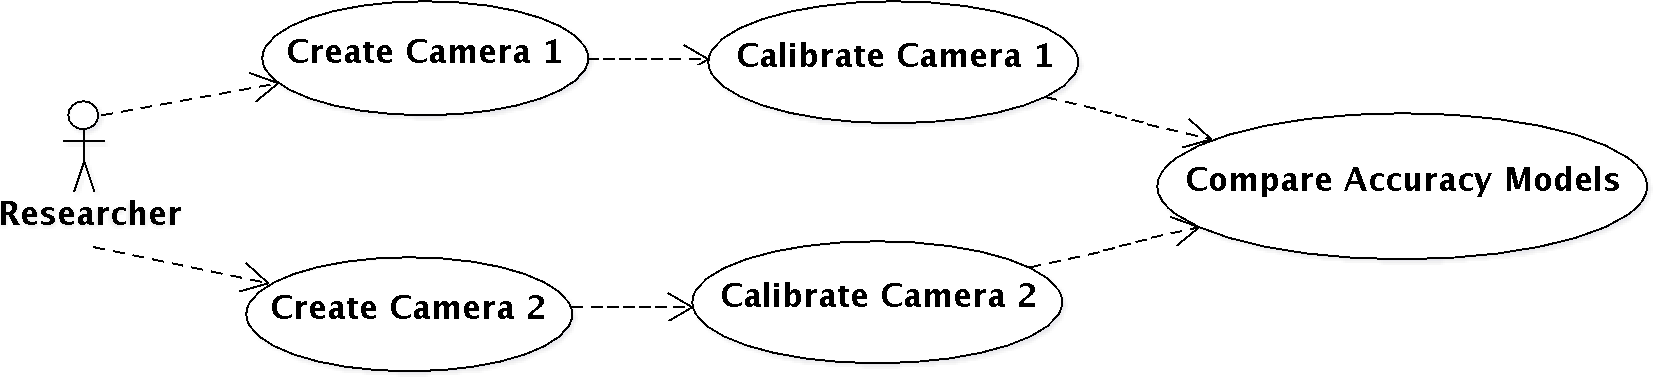
\includegraphics[scale=0.15]{images/CompareCameras.png}
    \caption{Researcher Use Cases}
    \label{fig:ucc}
    \end{figure}

    The Researcher user can perform calibration on two cameras and compare their accuracy models, to decided if they are suitable for their application. This use case is depicted in figure \ref{fig:ucc}.

\subsubsection{Training}

    \begin{figure}[htp]
    \centering
    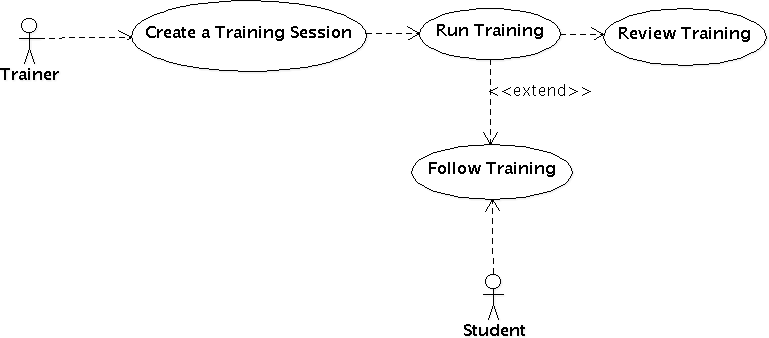
\includegraphics[scale=0.15]{images/Training.png}
    \caption{Generic Training User Cases}
    \label{fig:uco}
    \end{figure}

    Training involves two users. The Trainer can create a training session with a specified calibration procedure (camera, distortions, grid ... etc). Then the Trainer can send this session to a Student. 

    The Student will follow the Training Session and work towards a specified goal by the Trainer. The Student can also leave their feedback on completion that the Trainer can review, as described on \ref{fig:uco}

    The Student completes the training session by finishing camera calibration and sending back the camera distortion parameters, extrinsic and intrinsic values to the trainer. Additionally the student can record the difficulty level of the steps involved in 


\chapter{System Requirement Specifications}

\section{Calibration}
\subsection{Interface}

\section{Training}

The Trainer user can create a training session. A training session can consist of setting specific cameras, grids, and distortions. The trainer can then send a training plan to a student. 
The trainer will then review training. 
 
\subsection{Interface}
\subsection{Session}

\section{External Interface Requirements}

\subsection{Intact Robotics Haptics Arm}

\subsubsection{UDP Communications}

\subsubsection{High Level Interface}

\subsection{Graphical User Interface}

\section{Constraints}

\subsection{Reliability}

\subsection{Scalability}

\subsection{Performance}

\subsection{Security} 


\section{Functional Requirements}

\begin{enumerate}
\item Simulation
\begin{enumerate}
	\item Camera Model
	\item Camera Parameters 
\end{enumerate}
\end{enumerate}

\chapter{Next Steps}


\listoffigures 

\printglossaries

\bibliography{software_specs}{}

\end{document}
